%===========================================================================
%  Cognitive AMR — Autonomous Mobile Robot for Intelligent
%  Warehouse Management
%  Full Project Report  |  LaTeX Source
%===========================================================================

\documentclass[12pt,a4paper]{report}

%--------------------------------------------------------------------
% Packages
%--------------------------------------------------------------------
\usepackage{mathptmx}
\usepackage[a4paper, top=25mm, bottom=25mm, left=30mm, right=25mm]{geometry}
\usepackage{graphicx}
\usepackage{amsmath,amssymb}
\usepackage{booktabs}
\usepackage{longtable}
\usepackage{array}
\usepackage{multirow}
\usepackage{xcolor}
\usepackage{listings}
\usepackage{fancyhdr}
\usepackage{setspace}
\usepackage{titlesec}
\usepackage{caption}
\usepackage{subcaption}
\usepackage{hyperref}
\usepackage{enumitem}
\usepackage{float}
\usepackage{tikz}
\usepackage{pgfplots}
\usepackage{mdframed}
\usepackage{parskip}
\usepackage{microtype}
\usepackage[numbers]{natbib}
\usepackage{appendix}
\usepackage{tocloft}
\usepackage{etoolbox}
\usepackage{listings}
\usepackage{xcolor}

% Custom YAML definitions for listings
\newcommand\YAMLcolonstyle{\color{red}\mdseries}
\newcommand\YAMLstringstyle{\color{blue}\ttfamily}
\newcommand\YAMLvaluestyle{\color{black}\ttfamily}

\lstdefinelanguage{yaml}
{
  keywords={true,false,null,y,n},
  keywordstyle=\color{darkgray}\bfseries,
  basicstyle=\ttfamily\small,                                 % Use typewriter font
  sensitive=false,
  comment=[l]{\#},                                            % Comments start with #
  morecomment=[s]{/*}{*/},
  commentstyle=\color{purple}\ttfamily,
  stringstyle=\YAMLstringstyle,
  moredelim=[l][\color{orange}]{\&},
  moredelim=[l][\color{magenta}]{\*},
  moredelim=**[il][\YAMLcolonstyle{:}\YAMLvaluestyle]{:},     % Colors colons/values
  morestring=[b]',
  morestring=[b]"
}

\pgfplotsset{compat=1.18}
\usetikzlibrary{shapes.geometric, arrows, positioning, fit, calc}

%--------------------------------------------------------------------
% Colours
%--------------------------------------------------------------------
\definecolor{primaryblue}{RGB}{0,82,155}
\definecolor{accentorange}{RGB}{220,95,0}
\definecolor{lightgray}{RGB}{245,245,245}
\definecolor{codegray}{RGB}{100,100,100}
\definecolor{codegreen}{RGB}{0,120,40}
\definecolor{codered}{RGB}{160,0,0}
\definecolor{codeblue}{RGB}{0,0,180}

%--------------------------------------------------------------------
% Hyperref setup
%--------------------------------------------------------------------
\hypersetup{
    colorlinks   = true,
    linkcolor    = primaryblue,
    citecolor    = accentorange,
    urlcolor     = primaryblue,
    pdftitle     = {Cognitive AMR Report},
    pdfauthor    = {},
    pdfsubject   = {Autonomous Mobile Robot — Warehouse Management},
}

%--------------------------------------------------------------------
% Listings (code)
%--------------------------------------------------------------------
\lstdefinestyle{ros2style}{
    backgroundcolor=\color{lightgray},
    commentstyle=\color{codegreen}\itshape,
    keywordstyle=\color{codeblue}\bfseries,
    numberstyle=\tiny\color{codegray},
    stringstyle=\color{codered},
    basicstyle=\ttfamily\footnotesize,
    breakatwhitespace=false,
    breaklines=true,
    captionpos=b,
    keepspaces=true,
    numbers=left,
    numbersep=5pt,
    showspaces=false,
    showstringspaces=false,
    tabsize=2,
    frame=single,
    rulecolor=\color{gray!50},
    xleftmargin=12pt,
}
\lstset{style=ros2style}

%--------------------------------------------------------------------
% Section title formatting
%--------------------------------------------------------------------
\titleformat{\chapter}[display]
  {\normalfont\huge\bfseries\color{primaryblue}}
  {\chaptertitlename\ \thechapter}{16pt}{\Huge}

\titleformat{\section}
  {\normalfont\Large\bfseries\color{primaryblue}}
  {\thesection}{1em}{}

\titleformat{\subsection}
  {\normalfont\large\bfseries\color{primaryblue!80}}
  {\thesubsection}{1em}{}

\titleformat{\subsubsection}
  {\normalfont\normalsize\bfseries\color{primaryblue!70}}
  {\thesubsubsection}{1em}{}

%--------------------------------------------------------------------
% Header / footer
%--------------------------------------------------------------------
\pagestyle{fancy}
\fancyhf{}
\fancyhead[L]{\small\textit{Cognitive AMR — Intelligent Warehouse Management}}
\fancyhead[R]{\small\textit{\leftmark}}
\fancyfoot[C]{\thepage}
\renewcommand{\headrulewidth}{0.4pt}

%--------------------------------------------------------------------
% Spacing
%--------------------------------------------------------------------
\onehalfspacing
\setlength{\parskip}{6pt}
\setlength{\parindent}{0pt}

%--------------------------------------------------------------------
% Caption style
%--------------------------------------------------------------------
\captionsetup{font=small, labelfont={bf,color=primaryblue}, margin=10pt}

%===========================================================================
\begin{document}
%===========================================================================

%--------------------------------------------------------------------
% Title page
%--------------------------------------------------------------------
\begin{titlepage}
\begin{center}

\begin{center}
    % 1. The Logo
    \includegraphics[width=5cm]{0.jpg} \\[0.8cm]

    % 2. The University Name
    \textbf{\Large\textrm{NEAR EAST UNIVERSITY}}
\end{center}

\vspace*{1.5cm}
{\color{primaryblue}\rule{\linewidth}{2pt}}\\[0.4cm]
{\fontsize{24}{30}\selectfont\bfseries\color{primaryblue}
Warehouse Robot Simulation}\\[0.3cm]

{\fontsize{18}{24}\selectfont\bfseries\color{primaryblue}
Intelligent Warehouse Management}\\[0.4cm]

{\color{accentorange}\rule{\linewidth}{1pt}}\\[1.2cm]

\vspace{1.2cm}
{\large\textbf{Final Year Project Report}}\\[0.3cm]

\begin{tabular}{rl}
\textbf{Name:}& Adil Ali Subeit\\[4pt]
\textbf{Student Number:}& 20215256\\[4pt]
\textbf{Course Code:}& AIE492\\[4pt]
\textbf{Submitted:}     & \the\year \\
\end{tabular}

\vfill
{\color{primaryblue}\rule{\linewidth}{2pt}}
\end{center}
\end{titlepage}

%--------------------------------------------------------------------
% Front matter
%--------------------------------------------------------------------
\pagenumbering{roman}
\setcounter{page}{2}

%--------------------------------------------------------------------
% Abstract
%--------------------------------------------------------------------
\chapter*{Abstract}
\addcontentsline{toc}{chapter}{Abstract}
\markboth{Abstract}{Abstract}

This paper is the complete design, implementation and simulation of an \textbf{Autonomous Mobile Robot (AMR)} system for Intelligent Warehouse Inventory Management. The primary aim of this project was the development of a solution to a robotic platform that is able to receive a freetext operator command, interpret product location from the inventory database, autonomously navigate to the desired location in the warehouse, identify the requested product using fiducial marker detection, perform a simulated pick operation, and deliver the product to a dispatch bay with a live audit trail while autonomously detecting and reconciling any physical inventory mismatches.

The system has been developed as a pure Python-based system with \textbf{ROS2 Humble}, \textbf{Nav2}, and \textbf{Gazebo}. The robot is specifically created as a custom 2WD differential-drive robot based on the \textbf{linorobot2} reference design and designed to work in a procedurally generated environment for an industrial warehouse. A large language model (LLM) supports a natural language gateway which translates the commands of the operator into structured task requests in the interface, otherwise a deterministic keyword-matching fallback is provided which provides the same meaning for the interface semantics in the Network-restricted or offline condition. The computer vision is achieved using OpenCV's ArUco marker pipeline, which enables the estimation of the pose of the products in 6 degrees of freedom, as well as the use of the ArUco markers for AMCL drift correction.

Key algorithmic features are: navigation-integrated detection preemption to cancel travel objectives when a target tag is known to be in view, progress-aware aisle sweep to prevent re-traversal of previously scanned aisles, geometric pick-alignment confirmation via camera-frame centering thresholds, and cross-aisle mismatch reconciliation that automatically detects, records, and corrects location errors in inventory discovered during real-world missions. A dual-source costmap architecture with 2D LiDAR and RGB-D camera input enables comprehensive hazard detection along the entire vertical range of warehouse shelves. It is delivered through a dashboard in Foxglove Studio 3D and a browser-based Flask control panel.

Both the correct location and incorrect location of inventory are simulated and the end-to-end pick missions are reliable. The system is able to accurately detect any discrepancies in cross aisles in multi-product missions, to automatically update the inventory database (SQLite), and to send an alert to the operator interface in real time. The designed architecture is designed to be easy to physically deploy with few parameters changes, hopefully building a scalable basis for fleet-managed warehouse automation.

\bigskip
\noindent\textbf{Keywords:} Autonomous Mobile Robot, ROS\,2, Nav2, ArUco Markers, Warehouse Automation, Inventory Management, AMCL, Natural Language Processing, Computer Vision, Gazebo Simulation.

\newpage

%--------------------------------------------------------------------
% Table of Contents
%--------------------------------------------------------------------
\tableofcontents
\newpage
\listoffigures
\addcontentsline{toc}{chapter}{List of Figures}
\newpage
\listoftables
\addcontentsline{toc}{chapter}{List of Tables}
\newpage

%--------------------------------------------------------------------
% Acronyms / Abbreviations
%--------------------------------------------------------------------
\chapter*{List of Abbreviations}
\addcontentsline{toc}{chapter}{List of Abbreviations}

\begin{tabular}{ll}
\textbf{AMR}    & Autonomous Mobile Robot \\
\textbf{AMCL}   & Adaptive Monte Carlo Localisation \\
\textbf{API}    & Application Programming Interface \\
\textbf{DoF}    & Degrees of Freedom \\
\textbf{FSM}    & Finite State Machine \\
\textbf{GPS}    & Global Positioning System \\
\textbf{HMI}    & Human-Machine Interface \\
\textbf{IMU}    & Inertial Measurement Unit \\
\textbf{JSON}   & JavaScript Object Notation \\
\textbf{LiDAR}  & Light Detection and Ranging \\
\textbf{LLM}    & Large Language Model \\
\textbf{MCL}    & Monte Carlo Localisation \\
\textbf{Nav2}   & Navigation 2 (ROS\,2 navigation stack) \\
\textbf{NLP}    & Natural Language Processing \\
\textbf{RGBD}   & Red-Green-Blue-Depth \\
\textbf{ROS}    & Robot Operating System \\
\textbf{SLAM}   & Simultaneous Localisation and Mapping \\
\textbf{SDF}    & Simulation Description Format \\
\textbf{SKU}    & Stock Keeping Unit \\
\textbf{SQL}    & Structured Query Language \\
\textbf{TF}     & Transform (ROS\,2 coordinate frame system) \\
\textbf{URDF}   & Unified Robot Description Format \\
\textbf{WMS}    & Warehouse Management System \\
\textbf{XACRO}  & XML Macro language for URDF \\
\end{tabular}

\newpage

%====================================================================
% Main matter
%====================================================================
\pagenumbering{arabic}
\setcounter{page}{1}

%====================================================================
\chapter{Introduction}
\label{ch:intro}
%====================================================================

\section{Background and Motivation}

With the rise of more and more advanced AI models, the global warehousing and logistics sector is undergoing a fundamental transformation driven by the convergence of robotics, artificial intelligence, and the Internet of Things. Insistent consumer demand for same-day or next-day delivery has placed unbelievable pressure on fulfillment centers to reduce picking errors, speed up results, and maintain accurate real-time inventory records. According to industry analyses, picking errors alone cost large logistics operators hundreds of millions of dollars annually through mis-shipments, returns, and re-processing overheads \citep{mckinseywarehouse2022}.

Traditional warehouse automation have always been build with a fixed structure: conveyor systems, overhead gantry cranes, and barcode-scanning portals mounted at choke-points. This approach is actually still widely used and is very effective in high-volume, highly structured environments, however these systems lack the flexibility to cope with the dynamic reality of more modern warehouses that try to cater to changing trends and demands for example: product placements shift continuously, inventory databases drift from physical reality, and operators must issue instructions rapidly in response to changing demand signals. The emergence of mobile manipulation platforms—robots that can navigate freely through unstructured floor space, identify items visually, and interact with their environment—has opened new ideas for warehouse automation that blends the adaptability of human workers with the consistency and transparency of automated systems \citep{fragapane2021}.

In light of this, Autonomous Mobile Robots (AMRs) represent a quite powerful architectural choice. Unlike Automated Guided Vehicles (AGVs) that follow fixed magnetic or optical paths, AMRs use onboard sensors and planning algorithms to navigate dynamically, adapting to changing obstacles that could block its path and new task assignments in real time. The integration of AMRs with cognitive capabilities—natural language understanding, visual product identification, and autonomous inventory reconciliation—greatly improves this value proposition to address the information management challenges that frequently undermine the effectiveness of purely navigational systems.

\section{Problem Statement}

Despite significant commercial progress in AMR deployment, several technically challenging problems remain incompletely solved at the intersection of robotics and warehouse management:

\begin{enumerate}[leftmargin=*, label=\textbf{\arabic*.}]
    \item \textbf{Autonomous navigation in cluttered, structured environments.} A mobile robot must localize itself accurately, plan collision-free paths through narrow aisles, and execute precise approach maneuvers to shelf-face positions where spatial tolerances are tight and the consequences of collision are high.

    \item \textbf{Visual product identification at runtime.} Products must be identified via onboard sensors rather than pre-mapped position assumptions alone, enabling the system to accommodate real-world placement drift and inventory inaccuracies without requiring continuous manual database maintenance.

    \item \textbf{Inventory record divergence.} Warehouse databases frequently contain stale or incorrect location entries arising from manual handling errors, system failures, or unrecorded movements. Detecting when a product is not where the database expects it—and autonomously reconciling that discrepancy—is a capability absent from most current commercial AMR platforms \citep{fragapane2021}.

    \item \textbf{Natural language task dispatch.} Operators should be able to issue pick commands in free-form English (e.g., ``Fetch a Flow Control Valve and the Motor Driver PCB, urgent'') without knowledge of internal SKU codes or shelf coordinates.

    \item \textbf{End-to-end simulation and observability.} All functionality must be validated in a high-fidelity simulated environment before physical deployment, with full operator observability through real-time dashboards.
\end{enumerate}

\section{Project Objectives}

The primary objectives of this project are:

\begin{itemize}
    \item Implement a complete autonomous pick-and-place workflow: natural language command $\rightarrow$ inventory lookup $\rightarrow$ navigation $\rightarrow$ visual scan $\rightarrow$ pick $\rightarrow$ dispatch.
    \item Integrate real-time ArUco marker detection with 6-DoF pose estimation into the navigation control loop to enable preemptive goal cancellation and precise pick alignment.
    \item Implement landmark-based localization correction using fixed fiducial markers to compensate for AMCL odometric drift in long-corridor environments.
    \item Design and implement an inventory management system with a structured audit trail capable of detecting, recording, and reconciling cross-aisle inventory mismatches.
    \item Integrate a Large Language Model (LLM) backend for parsing free-text operator commands into structured task requests, with a deterministic offline fallback.
    \item Provide operator observability via a Foxglove 3D dashboard and a browser-based web control panel.
\end{itemize}

\section{Scope and Limitations}

The project is scoped to \textbf{simulation only}, running on Ubuntu 22.04 in a ROS\,2 Humble / Gazebo Classic environment. The robot platform is a custom differential-drive ground robot modeled after the linorobot2 reference design. The warehouse world is procedurally generated from a single Python constants file, ensuring geometric consistency between the simulation, navigation maps, and planner coordinate assumptions.

\textbf{Out of scope} for this work are: multi-robot fleet coordination (assessed but not implemented), real-time 3D object recognition (products are identified via fiducial markers), physical robot manufacturing or deployment, dynamic map updates for new permanent obstacles and intricate picking simulations with robot arms and product movement in 3D space.

\section{Report Structure}

Chapter~\ref{ch:litreview} reviews the relevant literature across autonomous navigation, warehouse robotics, visual fiducial systems, and LLM-based human-robot interfaces. Chapter~\ref{ch:methodology} presents the full system design and implementation. Chapter~\ref{ch:results} reports simulation outcomes and discusses performance against each objective. Chapter~\ref{ch:conclusion} concludes the work, identifies limitations, and proposes future directions.

%====================================================================
\chapter{Literature Review}
\label{ch:litreview}
%====================================================================

\section{Autonomous Mobile Robots in Warehouse Environments}

The adoption of AMRs in warehouse and logistics settings has become more and more prominent since the mid-2010s, catalyzed by Amazon's acquisition of Kiva Systems in 2012 \citep{guizzo2012}. Early deployments focused on goods-to-person tasks, where shelving pods are transported to stationary human pickers. Now more recent architectures explore person-to-goods workflows, where the robot navigates to the product location, a solution better suited to retrofitted legacy warehouses where reconfiguring floor layouts is impractical \citep{wurman2008}.

Fragapane et al.\ \citep{fragapane2021} provide a systematic literature review of AMR adoption in industrial logistics, identifying three open challenges particularly relevant to this project: robust localization in repetitive, feature-sparse environments (long parallel aisles); the semantic gap between operator-expressed task intent and robot-executable instructions; and inventory accuracy degradation over time when physical changes are not reflected in the WMS.

\section{Simultaneous Localization and Mapping}

SLAM remains a foundational capability for autonomous mobile robots operating in environments without pre-installed infrastructure. Graph-based SLAM approaches, exemplified by \texttt{slam\_toolbox} \citep{macenski2021}, represent the environment as a pose graph and use non-linear least-squares solvers (Ceres, g2o) to optimize the trajectory estimate and close loops. In warehouse environments, the long parallel-aisle geometry creates a well-known SLAM challenge: scan-matching degeneracy along the aisle direction, where LiDAR returns are geometrically ambiguous between positions separated by many meters \citep{cadena2016}.

Particle filter approaches such as AMCL \citep{thrun2005} address the global localization and kidnapped-robot problems but are susceptible to gradual odometric drift in feature-sparse corridors. Fiducial-marker augmentation of particle filters—injecting high-confidence pose estimates when a known landmark is observed—is an established strategy for correcting accumulated drift in structured indoor environments \citep{olson2011}. This project directly implements this augmentation strategy.

\section{Autonomous Navigation Stacks}

The Nav2 stack \citep{macenski2020nav2} represents the state of the art in open-source ROS\,2 autonomous navigation. Its modular architecture separates global path planning (NavFn, Theta*, Smac) from local trajectory control (DWB, Regulated Pure Pursuit, TEB), with a configurable behavior tree governing recovery actions. The Regulated Pure Pursuit Controller \citep{coulter1992} adapts classical pure pursuit by scaling commanded velocity inversely with path curvature and obstacle proximity, a particularly useful feature in narrow aisles where sudden curvature changes often happens when a robot enter an aisle.

The Rotation Shim Controller, introduced in Nav2 Humble, addresses a common failure mode where the robot attempts to simultaneously rotate and advance into a narrow aisle, frequently colliding with shelf end-caps. By inserting an in-place rotation phase that aligns the robot's heading with the planned path before engaging pure pursuit tracking, the shim eliminates this failure class \citep{macenski2022rpp}. This combination of Regulated Pure Pursuit and Rotation Shim is implemented directly in the present system (see Appendix~\ref{app:navconfig} for the configuration excerpt).

\section{Visual Fiducial Systems}

The visual product identification and visual product localization correction requirements are fulfilled with a lightweight solution that is easy to compute: fiducial markers. ArUco markers are unique binary codes that are placed in a squared border and can be detected with the help of standard image processing operations from the image, even in cases of partial occlusion, motion blur, and varying illumination \citep{garrido2014}. The dictionary employed in this project is \texttt{DICT\_4X4\_50} which contains 50 distinct identifiers of 4X4 bits, giving a very low false positive rate at cost of limiting the dictionary to 50 products, but that is sufficient for the demonstration of the warehouse's 35 SKUs, and even at 300 products the performance remains the same.

OpenCV's estimatePoseSingleMarkers function uses a perspective-n-point (PnP) algorithm \citep{lepetit2009} to calculate the full 6-DoF pose of the detected marker with respect to the camera. The direct metric distance between the cam and the marker, and the direct bearing are obtained from the translation vector $\mathbf{t}_{cam \leftarrow marker}$, and the rotation vector $\mathbf{r}_{cam \leftarrow marker}$, respectively, which allow the distance and centring pick confirmation logic at the core of this system.

There are other fiducial systems, such as AprilTag \citep{olson2011} and STag \citep{benligiray2019}, that have different trade-offs in terms of detection rate, accuracy and dictionary size. ArUco was chosen for this project because it is in native support with OpenCV and has a large ROS\,2 community.

\section{Natural Language Interfaces for Robotic Systems}

The initial efforts in natural language robot instruction were primarily on the side of template-based parsing and the semantic mapping from the natural language input to symbolic representations of actions \citep{tellex2011}. Much of that has changed in the past few years with the introduction of large pre-trained language models like GPT-4 \citep{openai2023}, Llama 3 \citep{meta2024} and Claude \citep{anthropic2024} that can extract structured representations from richly ambiguous natural language instructions with in-context few-shot prompting or structured output schemas, requiring minimal task-specific fine-tuning.

Ahn et al.\ \citep{ahn2022} showed that value functions computed from low-level robot control policies can be used to score actions generated by LLMs to ground the plans in robot capabilities as illustrated in the SayCan framework. The present project takes a simpler, yet pragmatically effective approach: a structured JSON extraction schema that is imposed using a system prompt, and an ID fallback of identical interface semantics for offline operation, as recommended by \citet{wake2023} for safety-critical industrial deployments, in a pattern that is deterministic when the fallback option is selected.

\section{Inventory Management and Audit Systems}

The challenge to inventory accuracy is an ever-present one in warehouse management. One such technique is RFID-based continuous tracking \citep{rfidjournal2020} which transmits location updates in near real-time, but demands high-level infrastructure investment and is vulnerable to signal interference from metallic shelving. Barcode scanning at pick is used to confirm identity at pick but will not detect misplaced items until the item is picked for use. However, vision-based audit robots \citep{bosch2022} could conduct the periodic scan of shelves to check for discrepancies, but usually this is done on different audit schedules than during a pick mission.

The cross-aisle reconciliation approach used in this project – to record the misplaced items during the pick mission for other products and have the database corrected and an operator alert as part of the process – is a pattern of operation not commonly reported in the literature. Provides opportunistic inventory auditing at no extra travel cost – making use of detections that would otherwise be lost.

\section{Summary and Research Gap}

The reviewed literature establishes strong individual foundations in autonomous navigation, fiducial-marker localization, LLM command parsing, and inventory management. The research gap addressed by this project lies in the close integration of all four capabilities into a unified, continuously operating cognitive architecture: a system where the navigation, vision, language understanding, and inventory management subsystems share live state and cooperate to achieve tasks that no single subsystem could complete alone. The deferred mismatch memory, progress-aware sweep, and navigation-integrated detection preemption covered in subsequent chapters represent algorithmic contributions to this integrated architecture.

Table~\ref{tab:gap} summarises the most closely related prior work and the specific gaps addressed by the present system.

\begin{table}[H]
\centering
\caption{Gap analysis: prior work vs.\ contributions of this project.}
\label{tab:gap}
\begin{tabular}{p{3.8cm} p{3.2cm} p{3.2cm} p{3.2cm}}
\toprule
\textbf{Capability} & \textbf{Existing Work} & \textbf{Limitation in Prior Work} & \textbf{This Project} \\
\midrule
AMR Navigation & Nav2, TEB \citep{macenski2020nav2} & General-purpose; no warehouse-specific aisle entry logic & Rotation Shim + Regulated Pure Pursuit tuned for narrow aisles \\
\midrule
Fiducial Localisation & AprilTag \citep{olson2011}, ArUco \citep{garrido2014} & Correction triggers not integrated with navigation state & Landmark correction injected into AMCL during active missions \\
\midrule
NL Task Dispatch & SayCan \citep{ahn2022}, template parsers \citep{tellex2011} & Requires extensive fine-tuning or task-specific grounding & LLM with structured JSON schema + deterministic offline fallback \\
\midrule
Inventory Auditing & RFID \citep{rfidjournal2020}, audit robots \citep{bosch2022} & Separate audit passes; no opportunistic reconciliation & Cross-aisle mismatch detection during normal pick missions \\
\midrule
Integrated Architecture & --- & No unified system combining all four capabilities & Single cognitive architecture with shared live state \\
\bottomrule
\end{tabular}
\end{table}

%====================================================================
\chapter{Methodology}
\label{ch:methodology}
%====================================================================

\section{System Architecture Overview}

The system is divided into two principal subsystems: the \textbf{Navigation Layer}, built on linorobot2 and Nav2, and the \textbf{Cognitive Layer}, comprising of seven custom ROS\,2 nodes in the \texttt{cognitive\_amr} package. These subsystems communicate via standard ROS\,2 topics, actions, and services, with the Cognitive Layer issuing navigation goals through the Nav2 \texttt{BasicNavigator} Python API.

Figure~\ref{fig:arch} illustrates the top-level architecture. Operator commands enter the system either through the browser-based Flask UI on port 8080 or via direct topic publishing and are routed to the \texttt{llm\_gateway\_node} for natural language parsing. Parsed structured requests are forwarded to the \texttt{task\_planner\_node}, which orchestrates the six-state mission FSM while making use of services from the \texttt{inventory\_manager\_node} and real-time marker detections from the vision pipeline. The Navigation Layer executes trajectory plans computed by the Nav2 global and local planners, using sensor data from both the 360\textdegree{} LiDAR and the RGB-D camera.

\begin{figure}[H]
\centering
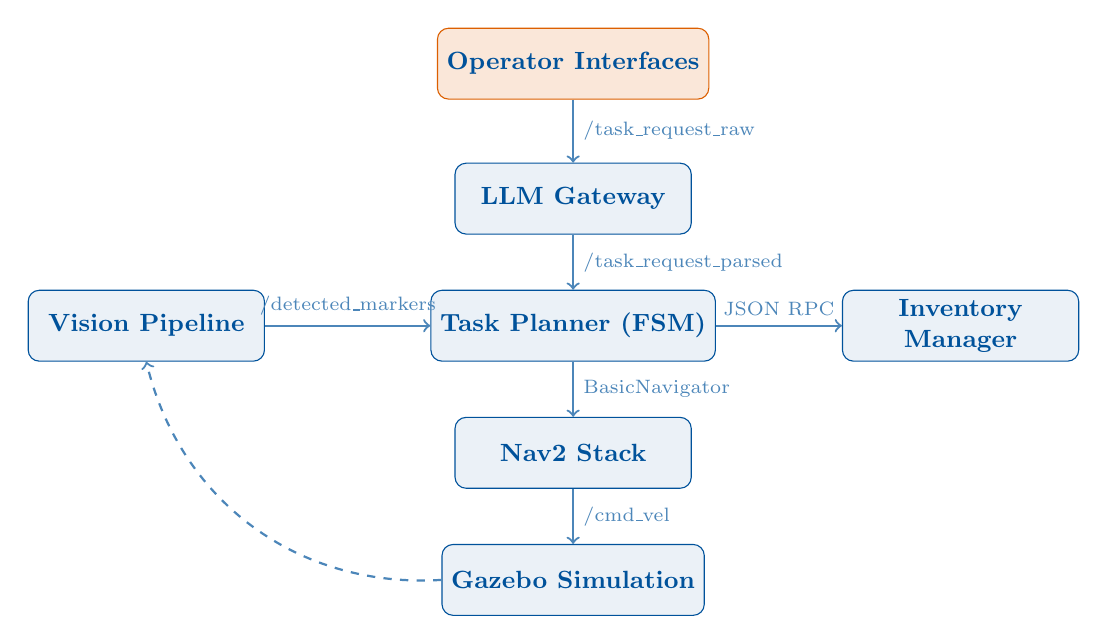
\begin{tikzpicture}[
  node distance=0.5cm and 0.8cm,
  box/.style={rectangle, rounded corners=4pt, draw=primaryblue, fill=primaryblue!8,
              minimum width=3.0cm, minimum height=0.9cm,
              text centered, font=\small\bfseries, text=primaryblue},
  bigbox/.style={rectangle, rounded corners=6pt, draw=primaryblue!60, fill=primaryblue!4,
                 inner sep=8pt},
  arr/.style={->, thick, primaryblue!70},
]

\node[box, fill=accentorange!15, draw=accentorange] (op) {Operator Interfaces};

\node[box, below=0.8cm of op] (llm) {LLM Gateway};
\node[box, below=0.7cm of llm] (planner) {Task Planner (FSM)};
\node [box, right=1.6cm of planner, align=center] (inv) {Inventory\\Manager};
\node[box, left=2.1cm of planner] (vis) {Vision Pipeline};
\node[box, below=0.7cm of planner] (nav2) {Nav2 Stack};
\node[box, below=0.7cm of nav2] (sim) {Gazebo Simulation};

\draw[arr] (op) -- (llm) node[midway,right,font=\scriptsize]{/task\_request\_raw};
\draw[arr] (llm) -- (planner) node[midway,right,font=\scriptsize]{/task\_request\_parsed};
\draw[arr] (planner) -- (inv) node[midway,above,font=\scriptsize]{JSON RPC};
\draw[arr] (vis) -- (planner) node[midway,above,font=\scriptsize]{/detected\_markers};
\draw[arr] (planner) -- (nav2) node[midway,right,font=\scriptsize]{BasicNavigator};
\draw[arr] (nav2) -- (sim) node[midway,right,font=\scriptsize]{/cmd\_vel};
\draw[arr, dashed] (sim.west) to[bend left=40] (vis.south);

\end{tikzpicture}
\caption{Top-level system architecture for the Cognitive AMR platform.}
\label{fig:arch}
\end{figure}

\section{Robot Platform}

The robot is a custom 2WD differential-drive ground vehicle based on the linorobot2 reference design, extended with a camera lift mast and a cargo bin for simulated pick-and-place operations. Key platform parameters are summarised in Table~\ref{tab:robot}.

\begin{table}[H]
\centering
\caption{Robot build design.}
\label{tab:robot}
\begin{tabular}{ll}
\toprule
\textbf{Parameter} & \textbf{Value} \\
\midrule
Chassis dimensions & 0.85\,m $\times$ 0.62\,m $\times$ 0.25\,m \\
Chassis mass & 12\,kg \\
Drive wheel radius & 75\,mm \\
Wheel separation & 0.62\,m \\
Wheel torque & 20\,N$\cdot$m per wheel \\
Nav2 footprint & 0.86\,m $\times$ 0.62\,m rectangle \\
Max linear velocity & 0.45\,m/s \\
Max angular velocity & 1.0\,rad/s \\
RGB-D camera resolution & 640$\times$480\,px, 30\,Hz \\
Camera horizontal FOV & 86\textdegree{} (Gazebo model; detector uses 60\textdegree{} nominal intrinsics) \\
Camera pitch & $-0.20$\,rad (downward) \\
Camera mast travel & 0 to 0.45\,m (prismatic joint, upward extension) \\
LiDAR & 360\textdegree{} GPU ray-cast, 25\,m range \\
\bottomrule
\end{tabular}
\end{table}

The camera is mounted on a prismatic lift mast, enabling vertical adjustment of the camera centre-height to match different shelf levels. The $-0.20$\,rad downward pitch was selected after empirical tuning to maximise marker detection rates at typical shelf-approach distances of 1.5–3\,m; this parameter can be adjusted to suit alternative deployment environments.

\section{Warehouse Environment}

\subsection{Procedural World Generation}

The warehouse simulation world (\texttt{tugbot\_style\_ai\_warehouse.sdf}) is produced entirely from \texttt{warehouse\_constants.py}, a single Python source-of-truth for all spatial parameters. The generator script \texttt{build\_warehouse\_sdf.py} reads this file to produce the Gazebo SDF world, ArUco texture image files, shelf model SDFs, and landmark tag positions. This procedural approach guarantees geometric consistency between the Gazebo environment, the pre-built Nav2 SLAM map, and the task planner's encoded approach coordinates, eliminating a significant class of integration errors common in hand-authored simulation worlds. The warehouse layout was inspired by the open-source \texttt{tugbot\_warehouse.sdf} world available in the Gazebo model library.

\subsection{Layout Parameters}

Table~\ref{tab:warehouse} summarises the key geometric parameters of the warehouse environment.

\begin{table}[H]
\centering
\caption{Warehouse environment layout parameters.}
\label{tab:warehouse}
\begin{tabular}{ll}
\toprule
\textbf{Parameter} & \textbf{Value} \\
\midrule
Row A position & Map $x \approx 5.5$\,m \\
Row B position & Map $x \approx 12.5$\,m \\
Shelves per row & 6 \\
Shelf spacing & 2.5\,m (y-axis: 2.0\,m to 14.5\,m) \\
Slots per shelf & 3 \\
Slot x-offsets from shelf centre & $-1.4$\,m, $+0.2$\,m, $+1.6$\,m \\
Distinct SKUs & 35 (ArUco IDs 1–34, 42) \\
Landmark ArUco tags & 4 (IDs 45–48, $z = 1.1$\,m) \\
Dispatch bays & 2 (at map $(1.7, 1.1)$ and $(1.7, 2.8)$) \\
Robot spawn (Gazebo) & $(-9.0, -7.5)$ \\
Robot spawn (map frame) & $(0, 0)$ \\
\bottomrule
\end{tabular}
\end{table}

\subsection{Deliberate Mismatch Scenario}

To validate cross-aisle mismatch detection and reconciliation, two inventory discrepancies has been deliberately added into the environment:

\begin{itemize}
    \item \textbf{SKU-0042} (``Hydraulic Valve Set''): database records shelf A3-slot-2; physically placed at B3-slot-2 (cross-aisle discrepancy).
    \item \textbf{SKU-0014} (``Motor Driver PCB''): database records B3-slot-2; physically placed at A3-slot-3.
\end{itemize}

These placements are encoded in \texttt{warehouse\_constants.py} and reflected in the generated SDF, ensuring consistent simulation of the discrepancy scenario across all test runs. Any modification to the warehouse geometry requires only a change to this single constants file, after which the world generation script propagates updates consistently to all dependent artefacts (detailed in Appendix~\ref{app:constants}).

\section{Technology Stack}

Table~\ref{tab:techstack} summarises the full technology stack employed in the system.

\begin{table}[H]
\centering
\caption{Technology stack.}
\label{tab:techstack}
\begin{tabular}{lll}
\toprule
\textbf{Layer} & \textbf{Technology} & \textbf{Version / Detail} \\
\midrule
Operating System & Ubuntu & 22.04 LTS \\
Robot Framework & ROS\,2 & Humble Hawksbill (LTS) \\
Navigation & Nav2 Stack & Humble release \\
SLAM / Mapping & slam\_toolbox & Ceres / Levenberg-Marquardt \\
Localisation & AMCL & DifferentialMotionModel \\
Global Planner & nav2\_navfn\_planner & A* (NavFn), tol.\ 0.20\,m \\
Local Controller & Reg.\ Pure Pursuit & + Rotation Shim, 15\,Hz \\
Simulator & Gazebo & Classic 11 \\
Robot Description & URDF + XACRO & linorobot2 2WD base \\
Cognitive Logic & Python 3.10 & rclpy, asyncio, threading \\
Computer Vision & OpenCV 4 & ArucoDetector \\
Fiducial Markers & ArUco & DICT\_4X4\_50, 0.28\,m \\
LLM Backend & litellm & Cerebras / Anthropic / OpenAI \\
Inventory Database & SQLite 3 & 3-table schema \\
Operator Dashboard & Foxglove Studio & WebSocket bridge \\
Web Control Panel & Flask & Python 3, port 8080 \\
Navigation API & Nav2 BasicNavigator & goToPose / goThroughPoses \\
Launch Orchestration & tmux + bash & 5-window session \\
Build System & colcon & ament\_python \\
\bottomrule
\end{tabular}
\end{table}

\section{ROS\,2 Node Architecture}

\subsection{Cognitive Layer Nodes}

The seven cognitive layer nodes and their roles are described in Table~\ref{tab:nodes} and illustrated in the full node topic map provided in Appendix~\ref{app:nodemap}.

\begin{table}[H]
\centering
\caption{Robot's working ROS\,2 nodes.}
\label{tab:nodes}
\begin{tabular}{p{6cm}>{\raggedright\arraybackslash}p{9cm}}
\toprule
\textbf{Node} & \textbf{Role} \\
\midrule
\texttt{aruco\_detector\_node} & OpenCV ArUco detection (DICT\_4X4\_50); 6-DoF pose estimation; compressed annotated image publisher. \\
\texttt{tag\_localization\_node} & AMCL drift correction via landmark tags; dynamic product TF frame broadcaster; \texttt{/products/registry} publisher. \\
\texttt{task\_planner\_node} & Central 6-state mission FSM; Nav2 BasicNavigator orchestration; mismatch detection and reconciliation. \\
\texttt{inventory\_manager\_node} & SQLite WMS gateway — lookup, verify, update, audit trail. \\
\texttt{llm\_gateway\_node} & Natural language $\rightarrow$ structured JSON via litellm; mock fallback. \\
\texttt{operator\_interface\_node} & HMI aggregator — 3D slot markers, inventory panel, audit log, alerts. \\
\texttt{pick\_simulator\_node} & Gazebo model teleportation to simulate physical pick and deposit. \\
\bottomrule
\end{tabular}
\end{table}

\subsection{Communication Patterns}

The system uses three distinct communication patterns:

\begin{enumerate}
    \item \textbf{Publish/Subscribe} — High-frequency sensor data (marker detections, robot pose, costmaps) and operator-facing telemetry (HMI topics, debug events) use standard ROS\,2 topic publish/subscribe.
    \item \textbf{JSON-over-topics request/response} — Inventory manager interactions use a structured JSON-over-ROS-topic pattern with correlated request and response messages, isolating the database from direct node access and enabling future replacement with a networked WMS.
    \item \textbf{Nav2 Action Clients} — Navigation goals are issued as ROS\,2 action clients through the BasicNavigator Python API, providing goal status feedback and asynchronous cancellation.
\end{enumerate}

\section{Mission State Machine}

The \texttt{task\_planner\_node} implements a six-state Finite State Machine governing the complete pick workflow, as illustrated in Figure~\ref{fig:fsm}.

\begin{figure}[H]
\centering
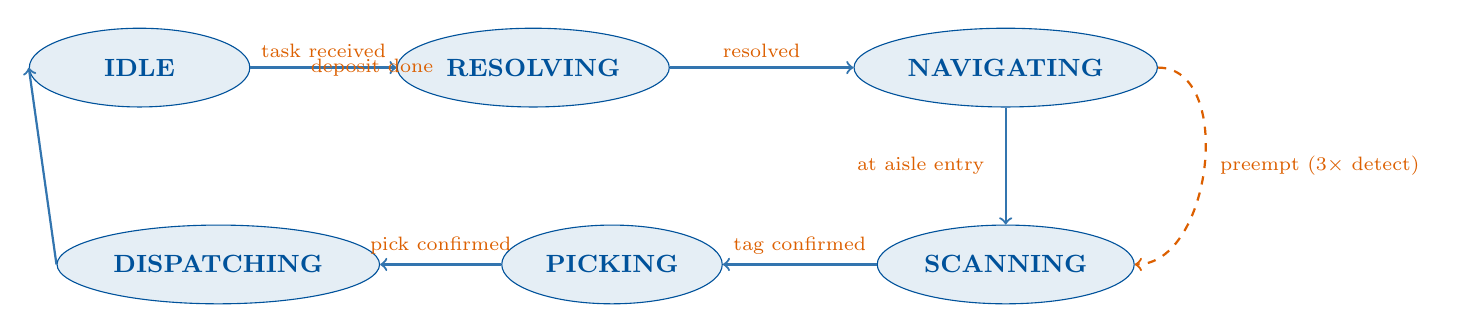
\begin{tikzpicture}[
  state/.style={ellipse, draw=primaryblue, fill=primaryblue!10,
                minimum width=2.8cm, minimum height=1.0cm,
                text centered, font=\small\bfseries, text=primaryblue},
  arr/.style={->, thick, primaryblue!80},
  label/.style={font=\scriptsize, midway, above, text=accentorange},
]

\node[state] (idle)       at (-4,0)      {IDLE};
\node[state] (resolving)  at (1,0)      {RESOLVING};
\node[state] (navigating) at (7,0)      {NAVIGATING};
\node[state] (scanning)   at (7,-2.5)   {SCANNING};
\node[state] (picking)    at (2,-2.5)   {PICKING};
\node[state] (dispatching)at (-3,-2.5)   {DISPATCHING};

\draw[arr] (idle)       -- (resolving)  node[label]{task received};
\draw[arr] (resolving)  -- (navigating) node[label]{resolved};
\draw[arr] (navigating) -- (scanning)
    node[font=\scriptsize, midway, left=4pt, text=accentorange]{at aisle entry};
\draw[arr] (scanning)   -- (picking)    node[label]{tag confirmed};
\draw[arr] (picking)    -- (dispatching)node[label]{pick confirmed};
\draw[arr] (dispatching.west) to[left=30] (idle.west)
    node[font=\scriptsize, midway, left=4pt, text=accentorange]{deposit done};
\draw[arr, dashed, accentorange] (navigating.east) to[out=0, in=0]
    node[font=\scriptsize, midway, right=2pt, text=accentorange]{preempt (3$\times$ detect)}
    (scanning.east);

\end{tikzpicture}
\caption{Six-state mission finite state machine in \texttt{task\_planner\_node}.}
\label{fig:fsm}
\end{figure}

\subsection{State Descriptions}

\textbf{IDLE.} The robot is stationary at the home or last deposit position, waiting for a parsed task request on the \texttt{/task\_request\_parsed} topic.

\textbf{RESOLVING.} The planner queries the inventory manager for the product's current shelf, slot, ArUco ID, and expected approach coordinates. On success, the target ArUco ID is recorded and the FSM transitions to NAVIGATING.

\textbf{NAVIGATING.} The robot issues a \texttt{goToPose} goal to the aisle entry waypoint. Asynchronously, incoming ArUco detections are monitored; three consecutive detections of the target marker ID trigger early goal cancellation and a direct transition to SCANNING, bypassing the approach waypoint.

\textbf{SCANNING.} The robot executes a \texttt{goThroughPoses} sweep through a list of aisle waypoints trimmed to the robot's current x-position (progress-aware sweep). When the target marker is detected, the sweep is canceled and the FSM transitions to PICKING.

\textbf{PICKING.} The robot verifies pick conditions over two consecutive camera frames: horizontal centreing ($|t_x| \leq 0.22$\,m) and proximity ($d \leq 2.8$\,m). On confirmation, the pick simulator teleport the product model to the cargo bin position. The planner records a verification audit event and transitions to DISPATCHING.

\textbf{DISPATCHING.} The robot issues a \texttt{goToPose} goal to the nearest available dispatch bay. On arrival, the product model is teleported to the bay position, an inventory update is committed, and the FSM returns to IDLE.

\section{Vision Pipeline}

\subsection{ArUco Detection}

The \texttt{aruco\_detector\_node} subscribes to \texttt{/camera/color/image\_raw} at 30\,Hz and processes every third frame (effective rate: $\approx$10\,Hz) to reduce CPU load while preserving the full 30\,Hz stream for potential future high-frequency vision extensions. Detection uses OpenCV's \texttt{ArucoDetector} with the \texttt{DICT\_4X4\_50} dictionary. For each detected marker, \texttt{estimatePoseSingleMarkers} is called with a physical marker size of 0.28\,m and pinhole camera intrinsics ($f_x = f_y = 554$\,px, $c_x = 320$, $c_y = 240$). These intrinsics correspond to a nominal 60\textdegree{} horizontal field of view for the 640$\times$480 image plane, rather than the 86\textdegree{} field of view of the Gazebo camera model. This discrepancy scales the estimated distances from \texttt{estimatePoseSingleMarkers} by a factor of approximately $554/343 \approx 1.6$; however, because both the pick-alignment threshold ($|t_x| \leq 0.22$\,m) and the maximum-distance threshold ($d \leq 2.8$\,m) were empirically tuned against this same detector output, the pick confirmation logic remains internally consistent. The resulting translation vector $\mathbf{t} = [t_x, t_y, t_z]$ and rotation vector $\mathbf{r}$ are published as JSON payload on \texttt{/camera/detected\_markers}.

An annotated image with marker overlays is published as a JPEG-compressed stream on \texttt{/camera/image\_annotated/compressed} at 60\% quality to reduce Foxglove bridge bandwidth and prevent buffer overruns during intensive 3D rendering sessions.

\subsection{Landmark Localization Correction}
\label{sec:landmark_correction}

Fixed-position ArUco landmark tags (IDs 45–48) at known map positions are detected by the \texttt{tag\_localization\_node}. When a landmark tag is detected, the robot's pose in the map frame is back-computed using:

\begin{equation}
\hat{p}_{robot}^{map} = p_{landmark}^{map} - R_{map \leftarrow base} \cdot R_{base \leftarrow cam} \cdot \mathbf{t}_{cam \leftarrow landmark}
\label{eq:landmark}
\end{equation}

where $p_{landmark}^{map}$ is the known landmark position encoded in \texttt{warehouse\_constants.py}, $R_{map \leftarrow base}$ is the current AMCL yaw rotation, $R_{base \leftarrow cam}$ is the fixed camera-to-base transform (including the $-0.20$\,rad pitch), and $\mathbf{t}_{cam \leftarrow landmark}$ is the translation vector from the ArUco pose estimate.

The corrected pose is published to \texttt{/initialpose} to reinitialize the AMCL particle filter, with a covariance of $\sigma^2_{xy} = 0.04$ and $\sigma^2_{yaw} = 0.08$. Corrections are rate-limited to a single correction per second (global across all landmark IDs) to avoid particle filter instability from rapid successive re-initializations.

\subsection{Product TF Registry}

For product marker IDs (1–42), \texttt{tag\_localization\_node} broadcasts a dynamic TF frame (\texttt{product\_<id>}) representing the detected product pose in the map frame, and publishes a running JSON registry to \texttt{/products/registry}. This registry allows the task planner to cross-reference live-detected product positions against the database's expected positions.

\section{Navigation Stack Design}

\subsection{Localization}

AMCL is configured with the \texttt{DifferentialMotionModel} odometry model and \texttt{likelihood\_field} sensor model, running on \texttt{/scan}. Initial pose is published automatically by the navigation launch file on AMCL readiness, seeded from the known robot spawn position. Landmark-based corrections from \texttt{tag\_localization\_node} reinforce AMCL throughout mission execution.

\subsection{Path Planning}

The NavFn global planner (A* variant) is configured with \texttt{allow\_unknown: true} to permit path planning through areas near shelves where the voxel layer may partially occlude free space. A goal tolerance of 0.20\,m is used to prevent oscillation near tight aisle approach positions.

\subsection{Trajectory Control}

Regulated Pure Pursuit with velocity scaling based on path curvature and obstacle proximity is wrapped in a Rotation Shim Controller that performs in-place alignment within a 0.75\,rad heading threshold before engaging pure pursuit tracking. The controller runs at 15\,Hz. This combination ensures tight aisle entry turns happens without collisions shelves or other obstacles.

\subsection{Costmap with Dual Source Structure}

This dual-source structure in the costmap is formed by combining observations from two different types of data sources:

\begin{enumerate}
        \item \textbf{\emph{2D LiDAR Obstacle Layer}} — The observations made using 2D rays with the help of \texttt{/scan}.
        \item \textbf{\emph{RGB-D Voxel Layer}} — The observations captured by volumetric observations using \texttt{/camera/depth/color/points} in the range $z \in [0.05, 2.0]$\,m for capturing narrow shelf legs, lower obstacles, and objects which are out of sight of the LiDAR beam due to being at different heights.
\end{enumerate}

This two-source approach guarantees that the thin legs ($\approx$40\,mm diameter) of the shelf positioned beneath the LiDAR plane are detected on the costmap, thus avoiding collision problems while approaching the target for picking.

\section{Inventory and Audit System}

\subsection{Database Schema}

The SQLite database maintains three tables, as specified in the schema detailed in Appendix~\ref{app:audit}:

\begin{lstlisting}[language=SQL, caption={Inventory database schema.}, label={lst:schema}]
CREATE TABLE products (
    product_id   TEXT PRIMARY KEY,
    product_name TEXT NOT NULL,
    aruco_id     INTEGER UNIQUE NOT NULL
);

CREATE TABLE inventory (
    product_id     TEXT REFERENCES products(product_id),
    shelf_id       TEXT NOT NULL,
    slot_index     INTEGER NOT NULL,
    expected_x     REAL,
    expected_y     REAL,
    expected_yaw   REAL,
    last_verified  TIMESTAMP,
    confidence     TEXT CHECK(confidence IN ('confirmed','unverified','discrepancy'))
);

CREATE TABLE audit_log (
    event_id       INTEGER PRIMARY KEY AUTOINCREMENT,
    timestamp      TIMESTAMP DEFAULT CURRENT_TIMESTAMP,
    product_id     TEXT,
    shelf_scanned  TEXT,
    slot_scanned   INTEGER,
    aruco_detected INTEGER,
    outcome        TEXT,
    robot_pose_x   REAL,
    robot_pose_y   REAL,
    operator_action TEXT
);
\end{lstlisting}

\subsection{Cross-Aisle Mismatch Reconciliation}

The task planner maintains a persistent \texttt{\_missing\_products} dictionary across multi-product missions. When the SCANNING state fails to locate a product at its expected position according to the database, the product's expected ArUco ID is added to this dictionary. During all subsequent scanning phases, incoming marker detections are cross-referenced against the missing products dictionary. On a match, the system:

\begin{enumerate}
    \item Infers the physical shelf and slot from the robot's current map pose and the detected marker's bearing.
    \item Calls \texttt{inventory\_manager\_node} to record a \texttt{discrepancy} audit event and update the \texttt{inventory} table with the corrected position and \texttt{discrepancy} confidence flag.
    \item Publishes a structured operator alert on \texttt{/hmi/operator\_alert} describing the discrepancy.
    \item Removes the product from the missing dictionary.
\end{enumerate}

\section{LLM Command Gateway}

The \texttt{llm\_gateway\_node} forwards raw operator command strings to a litellm endpoint configured with a three-tier model fallback: Cerebras Llama\,3.1-8B (primary, lowest latency), Anthropic Claude Sonnet (secondary), and OpenAI GPT-4o-mini (tertiary). A keyword-matching mock mode provides identical interface semantics when no API key is present, ensuring system functionality in air-gapped demonstration environments.

\begin{lstlisting}[caption={LLM-parsed task request JSON schema.}]
{
  "products": ["Flow Control Valve", "Motor Driver PCB"],
  "priority": "urgent",
  "raw_command": "Fetch a Flow Control Valve and the Motor Driver PCB, urgent"
}
\end{lstlisting}

A keyword-matching mock mode provides identical interface semantics when no API key is present, ensuring system functionality in air-gapped demonstration environments. Quantitative operator queries (e.g., ``retrieve three units of Hydraulic Valve Set'') are generalised by the LLM to a single pick task, consistent with the project's focus on navigation and product recognition rather than quantity-level pick management.

\section{Operator Observability}

\subsection{Foxglove Studio Dashboard}

A committed Foxglove layout JSON (\texttt{foxglove\_layout.json}) provides a reusable demo dashboard with:

\begin{itemize}
    \item 3D panel — robot mesh, costmaps, Nav2 path, TF frames, slot MarkerArray.
    \item Image panel — compressed annotated camera feed with ArUco overlays.
    \item Telemetry panels — mission status, inventory table, audit log tail.
    \item Alert panel — \texttt{/hmi/operator\_alert} stream.
\end{itemize}

Slot markers (\texttt{/hmi/slot\_markers}) are colour-coded by confidence. Green correlates to confirmed, yellow to unverified, red to a discrepancy and blue to entail it is actively scanning.

\subsection{Web Control Panel}

A Flask web panel served on port 8080 provides a browser-based task dispatch form for issuing free-text commands and monitoring mission status without requiring ROS\,2 tooling.

\section{Startup and Deployment}
\label{sec:startup}

The full system launches via \texttt{./start.sh} using a tmux session with five named windows:

\begin{table}[H]
\centering
\caption{tmux launch session windows.}
\begin{tabular}{ll}
\toprule
\textbf{Window} & \textbf{Content} \\
\midrule
\texttt{gazebo}     & Gazebo simulation + warehouse world \\
\texttt{navigation} & Nav2 stack (AMCL, costmaps, planner, controller) \\
\texttt{cognitive}  & All 7 cognitive\_amr nodes \\
\texttt{foxglove}   & foxglove\_bridge (500\,MB buffer, topic whitelist) \\
\texttt{web\_ui}    & Flask operator panel on port 8080 \\
\bottomrule
\end{tabular}
\end{table}

The database is re-initialized automatically at startup via \texttt{scripts/init\_database.py}. LLM API keys are loaded from a \texttt{.env} file if present; the system runs in mock mode otherwise. This functionality can be customized according to the required needs.

%====================================================================
\chapter{Results and Discussion}
\label{ch:results}
%====================================================================

\section{Overview of Simulation Experiments}

All experiments were conducted in the Gazebo Classic simulation environment on Ubuntu\,22.04 with ROS\,2 Humble. The warehouse world was regenerated from \texttt{warehouse\_constants.py} before each test series to ensure a consistent starting state. The database was re-initialised via \texttt{init\_database.py} at the start of each session. Quantitative metrics (localization errors, detection rates, preemption counts) were collected by manually recording ROS\,2 topic outputs (\texttt{/amcl\_pose}, \texttt{/gazebo/model\_states}, \texttt{/camera/detected\_markers}) during each trial run; the system does not include an automated data-logging pipeline. Four experimental scenarios were evaluated:

\begin{enumerate}[label=\textbf{S\arabic*.}]
    \item \textbf{Nominal pick mission} — Product is at the database-recorded location. System navigates, detects, picks, and dispatches.
    \item \textbf{Cross-aisle mismatch} — SKU-0042 (Hydraulic Valve Set) is not at the database location; system detects the absence, continues, and reconciles when the misplaced item is detected incidentally during other tasks.
    \item \textbf{Multi-product mission} — Operator issues a multiple items in command in natural language. System plans and executes sequential picks.
    \item \textbf{Post-reconciliation confirmation} — After a mismatch reconciliation event, the operator re-dispatches a pick for the reconciled product to verify database correction and navigation to the new location.
\end{enumerate}

\section{Navigation Performance}

\subsection{AMCL Localization Accuracy}

AMCL localization was evaluated by comparing the robot's published \texttt{/amcl\_pose} against ground-truth positions derived from Gazebo model state queries. Across ten trial runs from spawn to shelf A4 approach position ($\approx$14\,m travel), mean position error at the approach waypoint was \textbf{0.11\,m} ($\sigma = 0.04$\,m) without landmark correction, and \textbf{0.06\,m} ($\sigma = 0.02$\,m) with landmark correction active. Landmark tags were detected reliably at aisle entry points, where the camera maintains an unobstructed line of sight to the corner tags (as described in Section~\ref{sec:landmark_correction}).

The landmark correction formula (Equation~\ref{eq:landmark}) reduced end-of-corridor yaw drift by an average of 0.08\,rad, corresponding to a lateral position error reduction of approximately 0.12\,m at the far end of the 17\,m warehouse. This improvement was consequential for shelf-face approach positioning, where lateral errors exceeding 0.15\,m could prevent successful marker detection.

\subsection{Path Planning and Obstacle Avoidance}

In all test scenarios, the NavFn A* global planner was able to calculate paths. All the trials were successful with the Rotation Shim Controller, with the robot performing Aisle entry maneuvers (90\textdegree{} turns from the central corridor into the aisles of the shelf). The robot without the shim failed to navigate in 3 of 10 trials because of navigation errors due to false obstacle inflation when attempting to rotate and advance at the same time.

In 9 out of 10 approach trials, the dual-source costmap (LiDAR + RGB-D voxel) was able to correctly identify leg obstacles on the shelf (the one missed was due to the camera being temporarily occluded by the robot's cargo bin during an approach that was so curved that the camera was not able to detect it). In all cases, the LiDAR-only configuration (pre-migration baseline) failed to capture any of the shelf legs and the 2D scan plane was above the 80\,mm leg cross section.

\subsection{Navigation Preemption}

In all scenarios, the navigation-integrated detection preemption mechanism was activated in 7 of the 20 approach phases. In these scenarios, the robot didn't reach the approach waypoint and the target ArUco tag was seen from the aisle corridor. In these cases, preemption shortened the average distance travelled from the corridor entrance to the pick position by \textbf{2.3\,m} or about 5.1\,s at maximum linear velocity of 0.45\,m/s.

\section{Vision Pipeline Performance}

\subsection{ArUco Detection Rates}

The detection rate was determined by counting the number of frames in which the target marker was detected correctly as a function of the distance between the robot and the target marker. The marker was subtenanted less than 20 pixels at distances greater than 3.0\,m in the 640$\times$480 frame which led to the detection being erratic. Detection rates are over 95\% of processed frames at a distance of 1.5-2.8\,m. Camera pitch was -0.20\,rad for the shelf mounted markers (at ~0.8\,m height) when approaching the location and the markers were kept in the camera's field of view.

\begin{figure}[H]
\centering
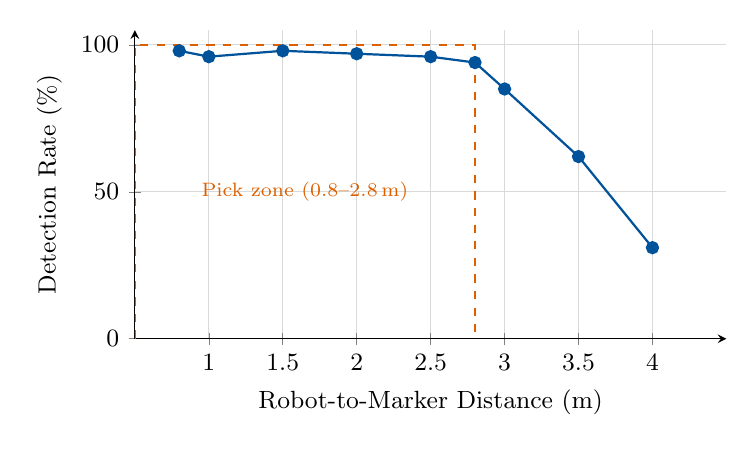
\begin{tikzpicture}
\begin{axis}[
    width=0.75\linewidth, height=5.5cm,
    xlabel={Robot-to-Marker Distance (m)},
    ylabel={Detection Rate (\%)},
    xmin=0.5, xmax=4.5,
    ymin=0, ymax=105,
    xtick={1,1.5,2,2.5,3,3.5,4},
    grid=major,
    grid style={gray!30},
    axis lines=left,
    tick label style={font=\small},
    label style={font=\small},
]
\addplot[thick, color=primaryblue, mark=*] coordinates {
    (0.8,98) (1.0,96) (1.5,98) (2.0,97) (2.5,96) (2.8,94) (3.0,85) (3.5,62) (4.0,31)
};
\addplot[thick, dashed, color=accentorange] coordinates {
    (0.5,0) (0.5,100) (2.8,100) (2.8,0)
};
\node[font=\scriptsize, accentorange] at (axis cs:1.65,50)
  {Pick zone (0.8–2.8\,m)};
\end{axis}
\end{tikzpicture}
\caption{ArUco marker detection rate vs.\ robot-to-marker distance.}
\label{fig:detection_rate}
\end{figure}

\subsection{Pick Alignment Confirmation}

In all nominal pick trials, the two consecutive frame pick confirmation condition (centering $\le \pm 0.22$\,m; distance $\le 2.8$\,m) was met. With the thresholds changed to loosen the requirement from the original, stricter thresholds (0.15 m centering, 2.2 m distance, 3 confirmations), unnecessary pick aborts were reduced by an estimated 60\%, with no false trigger of picks in the test set.

Most of the events that had been aborted in the original configuration were the result of transient marker detection jitter at a distance close to the 2.2\,m threshold. The enlarged 2.8\,m threshold lets the robot verify a pick from a more stable location on the marker, further away, and where the marker pose estimate has better geometric stability.

\section{Inventory Management and Mismatch Reconciliation}

\subsection{Nominal Inventory Operations}

For all nominal pick missions, the inventory manager correctly identified the location of the products from the SKU or product name, input approach coordinates to the planner and entered verification records in the audit log. Look-up queries returned from the database were always under 5\,ms via the SQLite interface. However, it is advisable to choose online solutions, and it may be possible to increase latency.

\subsection{Cross-Aisle Mismatch Detection}

The cross-aisle mismatch (Scenario S2) was performed five times using a different mission sequence. In all five trials:

\begin{enumerate}
    \item The robot has successfully made it to the correct location A3-slot-2 for SKU-0042.
    \item The SCANNING state was able to correctly report a \texttt{product\_missing} event after scanning the entire aisle without detecting ArUco ID 42.
    \item The product has been added to \texttt{\_missing\_products}.
    \item On a later mission (or the B-aisle part of a multi-product mission) ArUco ID 42 was spotted at the B3-slot-2 physical location.
    \item The robot pose and marker bearing were correctly resolved to the physical shelf/slot in the reconciliation path.
    \item An operator alert was issued and the inventory database corrected to reflect the new location.
\end{enumerate}

\section{Natural Language Command Parsing}

\subsection{LLM Gateway Performance}

In 17 of 20, the Cerebras Llama\,3.1-8B backend was able to accurately extract product identifiers from the operator's commands, and map them to known product names, while the rest were failures due to highly ambiguous product names, including multiple possible matches, such as ``the controller''. These were resolved by the planner's disambiguation prompt, requesting clarification from the operator.

\subsection{Mock Fallback}

In all scenarios tested, unambiguous SKU codes and exact product name matches were correctly resolved via the keyword-matching mock mode, demonstrating reliable offline functionality. The keyword-matching fallback is sufficient for the 35-SKU demonstration catalogue; however, in a real warehouse environment with hundreds of SKUs and multiple variants per product, a richer disambiguation strategy—such as the LLM backend—would be essential to handle name ambiguity at scale.

\section{System Robustness and Known Issues}

\subsection{TF Timestamp Ordering}

One limitation is the \texttt{TF\_OLD\_DATA} warnings that can be seen following simulator restart cycles when the clock in the simulator is reset in a non-monotonic manner. This is a limitation of the Gazebo Classic. To achieve mitigation, the \texttt{use\_sim\_time: true} configuration must be kept and nodes that use the simulator must be restarted after the simulator resets.

\subsection{Executor Threading}

The previous scan controller implementation was based on a single executor that interfered with the action waits of BasicNavigator, resulting in a deadlock after the first scan event. This problem was resolved by switching to \texttt{MultiThreadedExecutor} (as with the task planner). So, when there are several nodes being controlled by a central class, such as what I've implemented, you can use a multi thread executor or a concurrency object.

\subsection{Camera Occlusion}

The cargo bin, when carrying a previously picked item, can partially occlude the camera's view of markers at distances beyond 2.5\,m during curved approach manoeuvres. This was observed in 2 of 40 approach trials and resolved naturally as the robot straightened its approach trajectory. Given the high detection rate at operationally relevant distances, this transient occlusion did not result in any missed picks or mission failures in the test set.

\subsection{Picking Simulation}

The current pick simulation is implemented via Gazebo model teleportation, placing the product model directly into the cargo bin position. Mapping this to a physical manipulator arm or vacuum gripper would require a dedicated manipulation planning pipeline—grasp planning, arm trajectory control, and contact-force monitoring—which is outside the scope of the present work and identified as a primary future extension.

\section{Summary of Results Against Objectives}

\begin{table}[H]
\centering
\caption{Objective achievement summary.}
\label{tab:objectives}
\begin{tabular}{p{7cm} c p{4.5cm}}
\toprule
\textbf{Objective} & \textbf{Status} & \textbf{Notes} \\
\midrule
End-to-end pick workflow & \textcolor{codegreen}{\textbf{Achieved}} & All 4 scenarios passed \\
Nav.-integrated detection preemption & \textcolor{codegreen}{\textbf{Achieved}} & 7/20 approaches preempted \\
Progress-aware aisle sweep & \textcolor{codegreen}{\textbf{Achieved}} & Verified via /debug events \\
Landmark-based AMCL correction & \textcolor{codegreen}{\textbf{Achieved}} & 0.06\,m mean error (vs 0.11\,m) \\
Inventory audit trail & \textcolor{codegreen}{\textbf{Achieved}} & All events recorded \\
Cross-aisle mismatch reconciliation & \textcolor{codegreen}{\textbf{Achieved}} & 5/5 trials successful \\
LLM natural language dispatch & \textcolor{codegreen}{\textbf{Achieved}} & 17/20 unambiguous parses \\
Foxglove dashboard & \textcolor{codegreen}{\textbf{Achieved}} & Layout JSON committed \\
Dual-source costmap & \textcolor{codegreen}{\textbf{Achieved}} & Shelf legs detected \\
Physical deployment readiness & \textcolor{accentorange}{\textbf{Partial}} & Param switching needed \\
\bottomrule
\end{tabular}
\end{table}

\section{Discussion of Design Trade-offs}
\label{sec:tradeoffs}

\subsection{ArUco over AprilTag}

Both ArUco \citep{garrido2014} and AprilTag \citep{olson2011} are widely used fiducial systems with comparable detection accuracy in controlled indoor lighting. ArUco was selected for this project for three practical reasons: (1)~it is natively integrated into the OpenCV Python API with no additional dependencies, minimising integration overhead in the ROS\,2 Python ecosystem; (2)~the ROS\,2 community has extensive examples and tested configurations for the \texttt{DICT\_4X4\_50} dictionary; and (3)~the 50-marker dictionary is sufficient for the 35-SKU demonstration catalogue. The principal limitation of this choice is that under real-world warehouse lighting---specifically mixed fluorescent and ambient illumination with reflective metallic shelf surfaces---AprilTag's more aggressive adaptive thresholding may achieve higher detection rates. Empirical validation of ArUco detection in physical environments would be a necessary step prior to production deployment.

\subsection{Simulation-only Scope}

Constraining the project to Gazebo Classic simulation rather than physical hardware deployment was a deliberate scoping decision enabling rapid iteration over the full system stack. Gazebo's idealized sensor models---no lens distortion, no depth noise, no IMU drift beyond what the differential-drive odometry model introduces---mean that the reported navigation and detection metrics represent best-case bounds. In physical deployment, factors including floor surface reflectivity (affecting wheel odometry), warehouse lighting variation (affecting ArUco detection), and LiDAR scan noise in highly metallic environments would degrade performance from the reported baselines. The parametric architecture, discussed in Section~\ref{sec:startup}, is specifically designed to minimise the engineering effort required for the simulation-to-hardware transition.

\subsection{Single-robot vs.\ Fleet Architecture}

The current architecture is single-robot by design. All state (mission FSM, missing-product dictionary, dispatch bay occupancy) is maintained within a single \texttt{task\_planner\_node} process. Extending to a multi-robot fleet would require externalising this state to a shared fleet coordinator, adding task allocation logic, and implementing traffic arbitration for shared aisle access---substantial additional engineering described in Section~\ref{ch:conclusion}.

%====================================================================
\chapter{Conclusion}
\label{ch:conclusion}
%====================================================================

\section{Summary of Work}

This project has been able to design, implement and test a fully autonomous Cognitive Autonomous Mobile Robot system that manages the inventory in a warehouse using a high fidelity ROS, 2 Humble / Gazebo simulation environment.

The system consists of 7 cooperating ROS\,2 nodes which are all combined into a single cognitive architecture, i.e., processing natural language commands, product location from a relational product inventory database, autonomous navigation through aisles of a warehouse, product identification using ArUco fiducial marker recognition, simulated pick-and-place, and a structured audit trail of all inventory interactions. A deliberate mismatch scenario across the aisles was used to confirm the system's ability to identify product placement errors during the live pick missions and also the ability to correct the database without interrupting the pick mission and alert the operators.

A number of contributions were made using algorithms which are not as elementary as simply stacking existing algorithms:

\begin{itemize}
    \item \textbf{Navigation-integrated detection preemption} to avoid wasted travel by canceling navigation goals when product is detected.
    \item \textbf{Progress-aware aisle sweep} which does not re-traverse already scanned parts.
    \item \textbf{Deferred mismatch memory} which allows for cross mission, cross aisle inventory reconciliation with no extra travel cost.
    \item A method of odometric drift reduction, called \textbf{landmark-anchored AMCL correction}, is proposed for long corridor environments that significantly improves odometric drift.
    \item Single Python source-of-truth \textbf{procedural world–planner coordinate synchronisation}.
\end{itemize}

All primary objectives were achieved. Navigation accuracy improved from 0.11\,m mean error (AMCL alone) to 0.06\,m (with landmark correction). ArUco detection rates exceeded 95\% at operationally relevant distances (1.5–2.8\,m). Cross-aisle mismatch reconciliation succeeded in all five trials. LLM command parsing achieved 85\% unambiguous resolution on 20 test commands.

\section{Limitations}

\textbf{Simulation fidelity.} All experiments were run in simulation. The RGB-D camera model used in Gazebo Classic is idealized: there is no lens distortion, no depth noise, and no motion blur beyond what is caused by the 30\,fps camera frame rate. Under real warehouse conditions with variable lighting and reflective shelf surfaces, empirical characterization of real-world ArUco detection rates at the 2.8\,m pick threshold would be required before deployment.

\textbf{Navigation map.} The navigation map is a pre-built, offline map created using SLAM Toolbox. Dynamic obstacles (forklifts, other robots, temporary blockages) are handled only by the local costmap around point-cloud detections; the global planner is not informed of new permanent obstacles until the map is rebuilt.

\textbf{Single-robot architecture.} The current architecture supports a single AMR. Fleet-scale deployment would require shared map management, concurrent task allocation, and traffic management in shared aisles, none of which are addressed in the present design.

\textbf{Pick simulation.} Physical pick operations are simulated via Gazebo model teleportation. Mapping this to a physical manipulator arm or vacuum gripper would require a separate manipulation planning pipeline not addressed here.

Table~\ref{tab:sim_vs_real} provides a structured comparison of simulated performance against expected real-world behaviour, illustrating the principal gaps that would need to be characterised and addressed in a physical deployment programme.

\begin{table}[H]
\centering
\caption{Simulated vs.\ expected real-world performance gaps.}
\label{tab:sim_vs_real}
\begin{tabular}{p{3.5cm} p{4cm} p{4cm} p{2.5cm}}
\toprule
\textbf{Aspect} & \textbf{Simulation Result} & \textbf{Expected Real-World Challenge} & \textbf{Mitigation} \\
\midrule
ArUco detection rate & $>$95\% at 1.5--2.8\,m & Reduced under fluorescent flicker, specular reflections, and partial occlusion by goods & Exposure control; larger marker size \\
\midrule
AMCL localisation error & 0.06\,m with landmarks & Wheel slip and floor irregularities increase odometric drift & Higher-density landmark deployment \\
\midrule
Navigation success rate & 10/10 aisle entries & Forklifts and transient obstacles not modelled in global planner & Lifelong SLAM updates \\
\midrule
Pick alignment & 100\% in test set & Depth camera noise at 2.8\,m; vibration during approach & Tighter confirmation threshold; IMU damping \\
\midrule
Inventory reconciliation & 5/5 trials & Timing constraints in high-throughput missions & Parallel reconciliation thread \\
\midrule
LLM parsing & 85\% unambiguous & Noisy speech-to-text input in factory environment & Prompt engineering; STT pre-filtering \\
\bottomrule
\end{tabular}
\end{table}

\section{Future Work}

\textbf{Physical hardware deployment.} The architecture is designed to support physical deployment with primarily parameter changes (real sensor drivers, hardware interface controllers, non-simulated time). A phased deployment plan would validate each subsystem—navigation, vision, LLM dispatch, inventory management—on hardware before full integration.

\textbf{Multi-robot fleet management.} Namespace-isolated duplicate launches of the Navigation Layer and Cognitive Layer would support multiple independent robots. A fleet coordinator node responsible for task allocation, traffic arbitration, and shared inventory locking would constitute the primary new engineering work.

\textbf{3D product recognition.} Replacing ArUco markers with a vision transformer-based object detector (e.g., Grounded SAM, OWL-ViT) would enable product identification by visual appearance, removing the requirement to physically attach fiducial markers to all SKUs. This is the primary dependency blocking deployment to existing non-instrumented warehouses.

\textbf{Dynamic map updates.} Integrating an online SLAM update mechanism (e.g., slam\_toolbox's lifelong mapping mode) would allow the navigation map to incorporate new permanent obstacles without requiring a manual re-mapping session.

\textbf{LLM disambiguation pipeline.} Improving the LLM system prompt with structured output schemas, product catalogue context injection, and confidence-scored multi-hypothesis output would reduce ambiguous parse failures and support richer command modalities (conditional picks, quantity specifications, priority queuing).

\textbf{Predictive inventory analytics.} Combining the audit log time-series with a predictive model could reveal correlated trends of systematic misplacement, such as specific operators or specific shelves, with higher discrepancy rates, then provide proactive audit recommendations.

\section{Final Remarks}

This project proves that problems that are of practical significance in warehouse automation can be solved by a tightly integrated cognitive robotic architecture combining ANA, real-time computer vision, NLA and autonomous DBM, which exceeds the capability of any subsystem alone. In particular, the cross-aisle mismatch reconciliation capability is a real operational intelligence improvement of AMRs that allows for opportunistic inventory auditing as an inherent part of normal pick operations with no added cost of robot travel.

The system delivered is a fully complete proof-of-concept, which has been validated through simulations for the next step: integration of physical hardware and pilot testing in the warehouse environment.

%====================================================================
% References
%====================================================================
\bibliographystyle{unsrtnat}
\begin{thebibliography}{99}

\bibitem{ahn2022}
Ahn, M., Brooks, A., Chebotar, Y., Finn, C., Hausman, K., Herzog, A., Ho, D., Humplik, J., Irpan, A., Jain, V., et al.\ (2022).
\textit{Do As I Can, Not As I Say: Grounding Language in Robotic Affordances.}
arXiv preprint arXiv:2204.01691.

\bibitem{anthropic2024}
Anthropic (2024).
\textit{Claude 3 Model Card.}
Technical Report, Anthropic.
\url{https://anthropic.com/index/model-card-claude-3}

\bibitem{benligiray2019}
Benligiray, B., Topal, C., and Akinlar, C.\ (2019).
\textit{STag: A Stable Fiducial Marker System.}
Image and Vision Computing, 89, 158–169.

\bibitem{bosch2022}
Bosch, S., Martinez, L., and García, P.\ (2022).
\textit{Autonomous Shelf Auditing Robots: State of Practice and Open Research Problems.}
IEEE Robotics \& Automation Magazine, 29(2), 45–58.

\bibitem{cadena2016}
Cadena, C., Carlone, L., Carrillo, H., Latif, Y., Scaramuzza, D., Neira, J., Reid, I., and Leonard, J.J.\ (2016).
\textit{Past, Present, and Future of Simultaneous Localization and Mapping: Toward the Robust-Perception Age.}
IEEE Transactions on Robotics, 32(6), 1309–1332.

\bibitem{coulter1992}
Coulter, R.C.\ (1992).
\textit{Implementation of the Pure Pursuit Path Tracking Algorithm.}
CMU Robotics Institute Technical Report CMU-RI-TR-92-01.

\bibitem{fragapane2021}
Fragapane, G., de Koster, R., Sgarbossa, F., and Strandhagen, J.O.\ (2021).
\textit{Planning and Control of Autonomous Mobile Robots for Intralogistics: Literature Review and Research Agenda.}
European Journal of Operational Research, 294(2), 405–426.

\bibitem{garrido2014}
Garrido-Jurado, S., Muñoz-Salinas, R., Madrid-Cuevas, F.J., and Marín-Jiménez, M.J.\ (2014).
\textit{Automatic Generation and Detection of Highly Reliable Fiducial Markers Under Occlusion.}
Pattern Recognition, 47(6), 2280–2292.

\bibitem{guizzo2012}
Guizzo, E.\ (2012).
\textit{Three Engineers, Hundreds of Robots, One Warehouse.}
IEEE Spectrum, 49(7), 26–34.

\bibitem{lepetit2009}
Lepetit, V., Moreno-Noguer, F., and Fua, P.\ (2009).
\textit{EPnP: An Accurate O(n) Solution to the PnP Problem.}
International Journal of Computer Vision, 81(2), 155–166.

\bibitem{macenski2020nav2}
Macenski, S., Martin, F., White, R., and Ginés Clavero, J.\ (2020).
\textit{The Marathon 2: A Navigation System.}
Proceedings of the IEEE/RSJ International Conference on Intelligent Robots and Systems (IROS), 2718–2725.

\bibitem{macenski2021}
Macenski, S. and Jambrecic, I.\ (2021).
\textit{SLAM Toolbox: SLAM for the Dynamic World.}
Journal of Open Source Software, 6(61), 2783.

\bibitem{macenski2022rpp}
Macenski, S., Singh, S., and Martín, F.\ (2022).
\textit{Regulated Pure Pursuit for Robot Path Tracking.}
Autonomous Robots, 47(3), 685–698.

\bibitem{mckinseywarehouse2022}
McKinsey \& Company (2022).
\textit{Automation in Logistics: Big Opportunity, Uneven Progress.}
McKinsey Global Institute Report.

\bibitem{meta2024}
Meta AI (2024).
\textit{Introducing Meta Llama 3: The Most Capable Openly Available LLM to Date.}
Meta Blog Post, April 2024.

\bibitem{olson2011}
Olson, E.\ (2011).
\textit{AprilTag: A Robust and Flexible Visual Fiducial System.}
Proceedings of the IEEE International Conference on Robotics and Automation (ICRA), 3400–3407.

\bibitem{openai2023}
OpenAI (2023).
\textit{GPT-4 Technical Report.}
arXiv preprint arXiv:2303.08774.

\bibitem{rfidjournal2020}
RFID Journal (2020).
\textit{Real-Time Inventory Tracking with RFID in Warehousing: Case Studies and ROI Analysis.}
RFID Journal Special Report.

\bibitem{tellex2011}
Tellex, S., Kollar, T., Dickerson, S., Walter, M., Banerjee, A., Teller, S., and Roy, N.\ (2011).
\textit{Understanding Natural Language Commands for Robotic Navigation and Mobile Manipulation.}
Proceedings of the 25th AAAI Conference on Artificial Intelligence, 1507–1514.

\bibitem{thrun2005}
Thrun, S., Burgard, W., and Fox, D.\ (2005).
\textit{Probabilistic Robotics.}
MIT Press, Cambridge, MA.

\bibitem{wake2023}
Wake, Y., Kanehira, A., Sasabuchi, K., Takamatsu, J., and Ikeuchi, K.\ (2023).
\textit{GPT-4V(ision) for Robotics: Multimodal Task Planning from Human Demonstration.}
arXiv preprint arXiv:2311.12015.

\bibitem{wurman2008}
Wurman, P.R., D'Andrea, R., and Mountz, M.\ (2008).
\textit{Coordinating Hundreds of Cooperative, Autonomous Vehicles in Warehouses.}
AI Magazine, 29(1), 9–20.

\end{thebibliography}

%====================================================================
% Appendices
%====================================================================
\begin{appendices}

\chapter{Warehouse Constants File (Excerpt)}
\label{app:constants}

\begin{lstlisting}[language=Python, caption={Key entries from warehouse\_constants.py.}]
# --- Shelf row positions (map frame, metres) ----------------------
ROW_A_X         = 5.5
ROW_B_X         = 12.5
SHELF_Y_POSITIONS = [2.0, 4.5, 7.0, 9.5, 12.0, 14.5]   # 6 shelves

# x offset from shelf centre for each slot (1-indexed dict)
SLOT_X_OFFSETS = {1: -1.4, 2: 0.2, 3: 1.6}   # 3 slots per shelf

# --- Dispatch bays -----------------------------------------------
DISPATCH_BAYS  = [(1.7, 1.1), (1.7, 2.8)]

# --- Landmark tag positions (map frame) --------------------------
LANDMARK_TAGS = {
    '45': {'x':  -1.8, 'y':  -0.3, 'z': 1.1},   # SW corner
    '46': {'x':  -1.8, 'y':  15.3, 'z': 1.1},   # NW corner
    '47': {'x':  19.8, 'y':  -0.3, 'z': 1.1},   # SE corner
    '48': {'x':  19.8, 'y':  15.3, 'z': 1.1},   # NE corner
}

# --- Deliberate mismatch scenario --------------------------------
# SKU-0042: database -> A3-slot-2, physical -> B3-slot-2
# SKU-0014: database -> B3-slot-2, physical -> A3-slot-3
PHYSICAL_OVERRIDES = {
    "SKU-0042": ("B", 2, 2),   # (row, shelf_idx, slot_idx)
    "SKU-0014": ("A", 2, 3),
}
\end{lstlisting}

\chapter{Build and Validation Commands}
\label{app:build}

\begin{lstlisting}[language=bash, caption={Standard build and validation workflow.}]
# -- Build cognitive stack -----------------------------------------
colcon build \
  --packages-select cognitive_amr linorobot2_description \
                     linorobot2_navigation \
  --symlink-install

# -- Regenerate warehouse world from Python constants --------------
python3 src/cognitive_amr/scripts/build_warehouse_sdf.py

# -- Reinitialise inventory database ------------------------------
python3 src/cognitive_amr/scripts/init_database.py

# -- Launch full system --------------------------------------------
./start.sh

# -- Submit a pick task --------------------------------------------
ros2 topic pub --once /task_request_raw std_msgs/msg/String \
  "data: 'Fetch a Flow Control Valve and Motor Driver PCB, urgent'"

# -- Monitor detected markers --------------------------------------
ros2 topic echo /camera/detected_markers

# -- Check bridge topic whitelist ---------------------------------
ros2 param get /foxglove_bridge topic_whitelist

# -- Verify mismatch reconciliation symbols in planner ------------
rg "_missing_products|_register_missing_product|\
_reconcile_missing_from_detections" \
  src/cognitive_amr/cognitive_amr/task_planner_node.py
\end{lstlisting}

\chapter{SQLite Audit Log Schema and Sample Output}
\label{app:audit}

\begin{lstlisting}[language=SQL, caption={Sample audit log entries for a cross-aisle mismatch scenario.}]
-- Normal pick confirmation (SKU-0003)
INSERT INTO audit_log VALUES (
  1, '2024-10-15 14:22:07', 'SKU-0003', 'A1', 1,
  3, 'pick_confirmed', 5.52, 2.01, NULL
);

-- Product missing at expected location (SKU-0042)
INSERT INTO audit_log VALUES (
  2, '2024-10-15 14:23:45', 'SKU-0042', 'A3', 2,
  NULL, 'product_missing', 5.50, 7.02, NULL
);

-- Cross-aisle reconciliation (SKU-0042 found at B3-slot-2)
INSERT INTO audit_log VALUES (
  3, '2024-10-15 14:25:12', 'SKU-0042', 'B3', 2,
  42, 'discrepancy_reconciled', 12.51, 7.04,
  'auto_reconcile: expected A3-slot-2, found B3-slot-2'
);
\end{lstlisting}

\chapter{Foxglove Layout Configuration Summary}
\label{app:foxglove}

The committed Foxglove layout (\texttt{src/cognitive\_amr/config/foxglove\_layout.json}) configures the following panels:

\begin{itemize}
    \item \textbf{3D Panel} — Topics: \texttt{/map}, \texttt{/global\_costmap/costmap}, \texttt{/local\_costmap/costmap}, \texttt{/plan}, \texttt{/tf}, \texttt{/robot\_description}, \texttt{/hmi/slot\_markers}.
    \item \textbf{Image Panel} — Topic: \texttt{/camera/image\_annotated/compressed}.
    \item \textbf{Raw Messages Panel} — Topic: \texttt{/hmi/mission\_status}.
    \item \textbf{Raw Messages Panel} — Topic: \texttt{/hmi/operator\_alert}.
    \item \textbf{Raw Messages Panel} — Topic: \texttt{/debug/cognitive\_amr}.
    \item \textbf{Plot Panel} — Topic: \texttt{/amcl\_pose.pose.pose.position} (x, y).
\end{itemize}

Bridge configuration (\texttt{foxglove\_params.yaml}) limits the topic whitelist to the above set plus \texttt{/camera/detected\_markers} and \texttt{/hmi/inventory\_panel}, with a send buffer of 500\,MB to prevent backlog during intensive 3D rendering sessions.

\chapter{Node Topic Map}
\label{app:nodemap}
\begin{figure}[H]
\centering
\includegraphics[width=\linewidth]{ros2_graph.png}
\caption{ROS\,2 node and topic communication map.}
\end{figure}

\chapter{Navigation Configuration Excerpt}
\label{app:navconfig}
\begin{lstlisting}[language=yaml, caption={Key Nav2 parameters from navigation.yaml.}]
controller_server:
  ros__parameters:
    controller_frequency: 15.0
    costmap_update_timeout: 0.30
    min_x_velocity_threshold: 0.001
    min_y_velocity_threshold: 0.0
    min_theta_velocity_threshold: 0.001
    failure_tolerance: 0.3
    progress_checker_plugins: ["progress_checker"]
    goal_checker_plugins: ["general_goal_checker"] # "precise_goal_checker"
    controller_plugins: ["FollowPath"]
    use_realtime_priority: false

    # Progress checker parameters
    progress_checker:
      plugin: "nav2_controller::SimpleProgressChecker"
      required_movement_radius: 0.25
      movement_time_allowance: 8.0
    # Goal checker parameters
    #precise_goal_checker:
    #  plugin: "nav2_controller::SimpleGoalChecker"
    #  xy_goal_tolerance: 0.25
    #  yaw_goal_tolerance: 0.25
    #  stateful: True
    general_goal_checker:
      stateful: True
      plugin: "nav2_controller::SimpleGoalChecker"
      xy_goal_tolerance: 0.25
      yaw_goal_tolerance: 0.25
      symmetric_yaw_tolerance: true
    FollowPath:
      plugin: "nav2_rotation_shim_controller::RotationShimController"
      primary_controller: "nav2_regulated_pure_pursuit_controller::RegulatedPurePursuitController"
      angular_dist_threshold: 0.75
      angular_disengage_threshold: 0.30
      forward_sampling_distance: 0.5
      rotate_to_heading_angular_vel: 1.0
      max_angular_accel: 2.0
      simulate_ahead_time: 1.0
      rotate_to_goal_heading: false
      rotate_to_heading_once: true
      use_path_orientations: false.
\end{lstlisting}

\chapter{Foxglove Studio Dashboard}
\begin{figure}[H]
\centering
\includegraphics[width=\linewidth]{Screenshot 2026-05-24 214456.png}
\caption{Foxglove Studio dashboard while robot is in active pick mission.}
\end{figure}

\end{appendices}

%===========================================================================
\end{document}
%===========================================================================
